
\section{EWS results}


The final binned fit is performed using the $m_T^I$ histogram for all signals and the number of events for the backgrounds.
For the oppiste-flavour and same-flavour analysis, for every categories and for every mass point from
200\GeV up to 3\TeV the significance  and the 95\% CL
upper exclusion limit are calculated.
The expected final limit from the combination of the OF and SF analysis are shown in fig. \ref{fig:lim_OFSF_comb}. 
This limit represent a 	considerable improvement respect to the high mass search done with 2015 data and the expected limits is compatible with the ATLAS results for a similar analysis (CERN-EP-2017-214; arXiv:1710.01123).\\

\begin{figure}[htb]
\centering
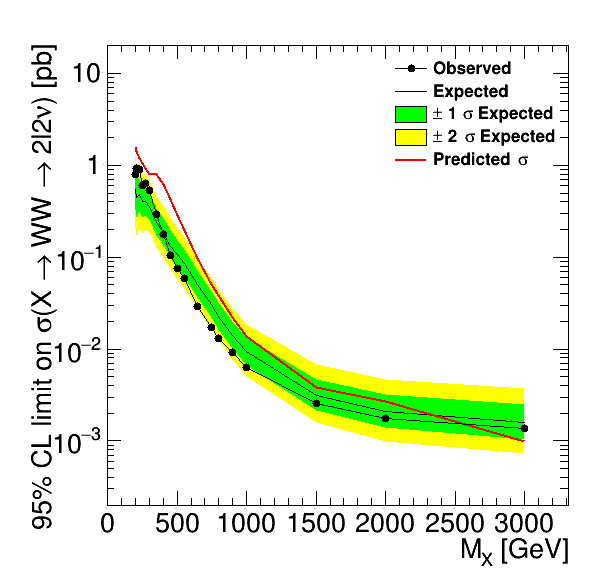
\includegraphics[width=0.65\textwidth]{../AN/Figs/unblinding/Limits/c2_FullComb_unbl.png}
\caption{95$\%$ CL exclusion limits,  on the production ggH and VBF cross section times branching fraction as a function of the mass for the { \bf combination} of the two analysis OF and SF, in the full mass range.   The red  line represent the predicted cross-section for EW high mass bosons.}

    \label{fig:sig_OFSF_comb_un}
\end{figure}





\subsection*{2HDM results}

In Fig. ~\ref{fig:MSSM} the exclusion limits are shown for the $m_h^{mod+}$ scenario on the left and the hMSSM scenario on the right. The dashed line marks the limit, while the green area shows the side of the limit that is excluded. The bands surrounding the limit indicate the $\pm 1,2\sigma$ contours. For both scenarios the region at low values of $m_{A}$ and $\tan\beta$ is excluded. These results complement well with the exclusion limit given by the MSSM $H\rightarrow\tau\tau$ analysis, where the sensitivity is lower for low $m_{A}$ and $\tan\beta$.

\begin{figure}[htb]
\centering
\subfigure[$m_h^{mod+}$]{
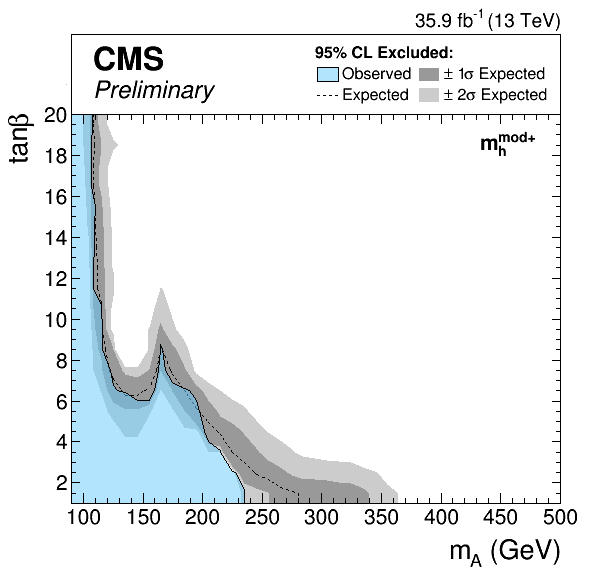
\includegraphics[width=0.45\textwidth]{../AN/Figs/unblinding/2HDM/mhmodp.png}
}
\subfigure[hMSSM]{
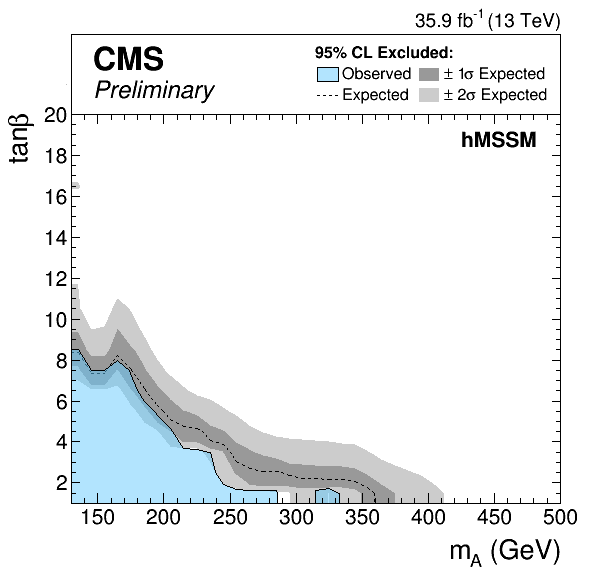
\includegraphics[width=0.45\textwidth]{../AN/Figs/unblinding/2HDM/hmssm.png}
}

\caption{95$\%$ CL exclusion limits on the MSSM $m_h^{mod+}$ scenario (left) and the hMSSM scenario (right).}
    \label{fig:MSSM}
\end{figure}

In Fig. ~\ref{fig:2HDM1} and ~\ref{fig:2HDM2} the exclusion limits are shown for a 2HDM. The limits in ~\ref{fig:2HDM1} for both a type-1 and type-2 2HDM is displayed in a $\cos(\beta-\alpha)$-$\tan\beta$ plane, in which the neutral heavy Higgs boson masses are $m_{H}=m_{A}=200$, $300$, $500\,$GeV and the convention $\sin(\beta-\alpha) > 0$ is used. The plots in Fig. ~\ref{fig:2HDM2} show the limit in the $m_{H}$-$\tan\beta$ plane. Here it is again assumed that $m_{H}=m_{A}$ and $\sin(\beta-\alpha) > 0$, but here the relationship between $\beta$ and $\alpha$ is $\cos(\beta-\alpha)=0.1$. The exclusion limits seen here are larger compared to those produced in the similar analysis by ATLAS. A possible reason may be the choice of the discriminating variable $m_{T}^{I}$ or the different categorization.

\begin{figure}[htb]
\centering
\subfigure[Type-1, $m_{H}=200\,$GeV]{
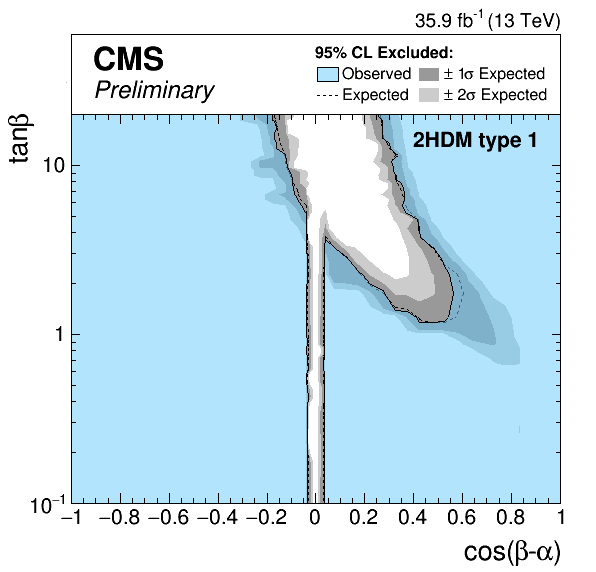
\includegraphics[width=0.45\textwidth]{../AN/Figs/unblinding/2HDM/thdm_cosba_t1_200.png}
}
\subfigure[Type-2, $m_{H}=200\,$GeV]{
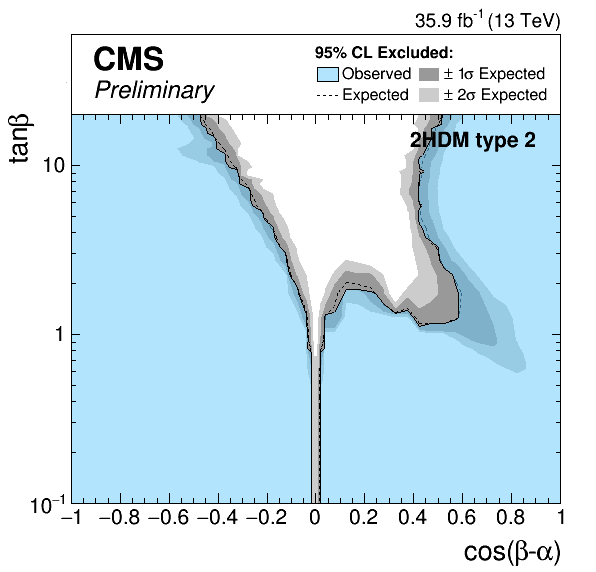
\includegraphics[width=0.45\textwidth]{../AN/Figs/unblinding/2HDM/thdm_cosba_t2_200.png}
}
\\
\subfigure[Type-1, $m_{H}=300\,$GeV]{
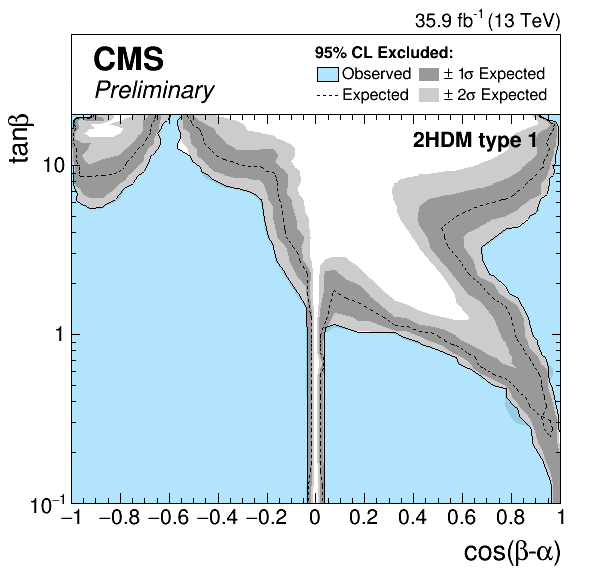
\includegraphics[width=0.45\textwidth]{../AN/Figs/unblinding/2HDM/thdm_cosba_t1_300.png}
}
\subfigure[Type-2, $m_{H}=300\,$GeV]{
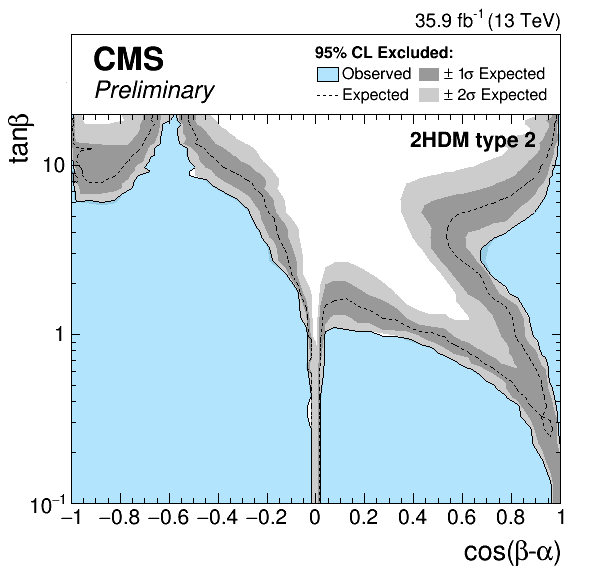
\includegraphics[width=0.45\textwidth]{../AN/Figs/unblinding/2HDM/thdm_cosba_t2_300.png}
}
\\
\subfigure[Type-1, $m_{H}=500\,$GeV]{
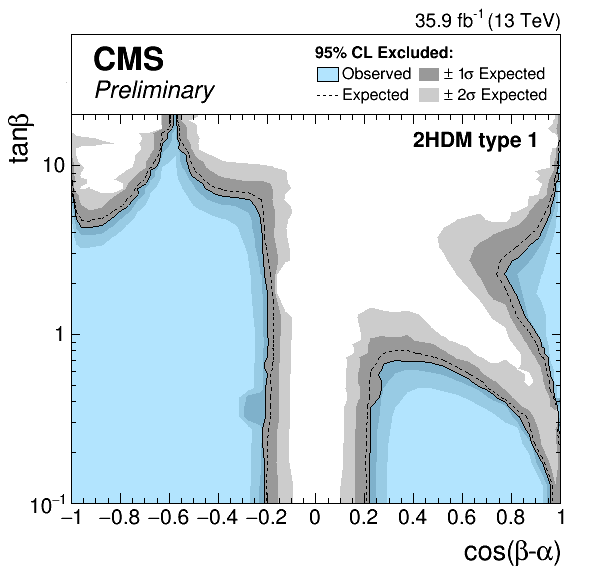
\includegraphics[width=0.45\textwidth]{../AN/Figs/unblinding/2HDM/thdm_cosba_t1_500.png}
}
\subfigure[Type-2, $m_{H}=500\,$GeV]{
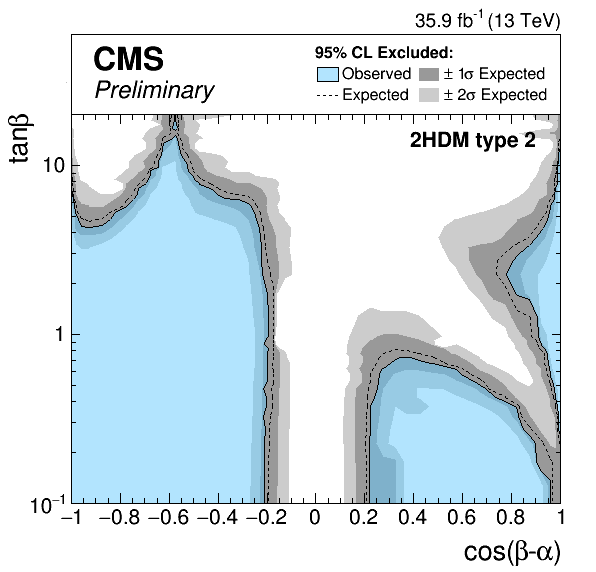
\includegraphics[width=0.45\textwidth]{../AN/Figs/unblinding/2HDM/thdm_cosba_t2_500.png}
}
\caption{95$\%$ CL exclusion limits on a 2HDM with $\cos(\beta-\alpha)$ on the x-axis. Limits are shown for a type-1 and type-2 2HDM for different masses $m_{H}=200$, $300$, $500\,$GeV.}
    \label{fig:2HDM1}
\end{figure}

\begin{figure}[htb]
\centering
\subfigure[Type-1, $\cos(\beta-\alpha)=0.1$]{
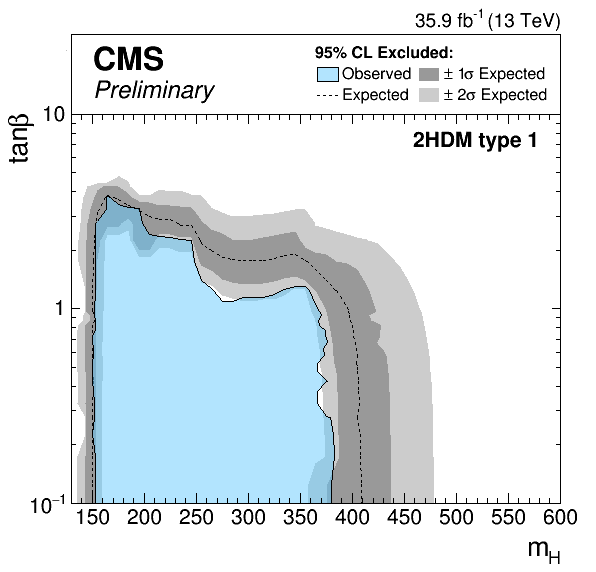
\includegraphics[width=0.45\textwidth]{../AN/Figs/unblinding/2HDM/thdm_mh_t1.png}
}
\subfigure[Type-2, $\cos(\beta-\alpha)=0.1$]{
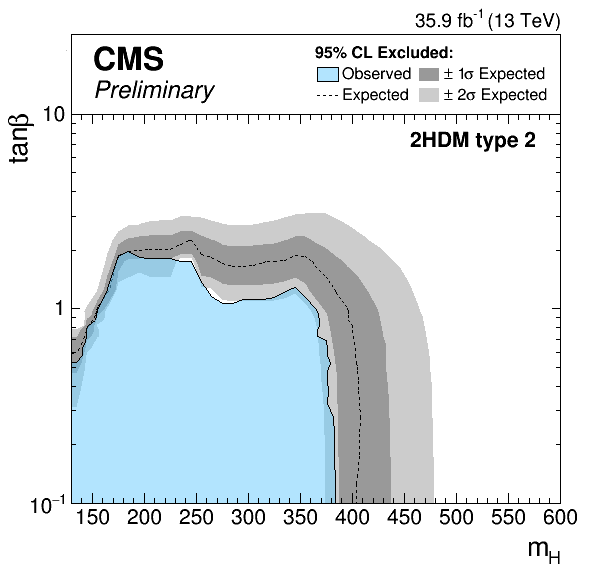
\includegraphics[width=0.45\textwidth]{../AN/Figs/unblinding/2HDM/thdm_mh_t2.png}
}

\caption{95$\%$ CL exclusion limits on a 2HDM with $m_{H}$ on the x-axis. Limits are shown for a type-1 and type-2 2HDM for $\cos(\beta-\alpha)=0.1$.}
    \label{fig:2HDM2}
\end{figure}

